%!TEX root = main.tex
\chapter{Preliminary Work}

Prior to the start of the development of TaleBlazer Analytics, many decisions had to be made in order to arrive at a feature specification for the system. In order to develop a useful analytics system, the types of analytics data to capture had to be determined. To meet the technical needs of the project, the technology used to build the new system had to be benchmarked and chosen. Finally, the user interface for the analytics site was mocked up and underwent an iterative design process.

\section{Types of Analytics Data to Capture}

The key purpose of TaleBlazer Analytics is to capture metrics about TaleBlazer games. In order to achieve this, it was first necessary to determine exactly what kinds of data would be useful to capture and if we could capture it. First, preliminary work was performed in TaleBlazer Mobile to identify the types of information that the system was to collect through the development of an additional mobile tab dedicated to logging information. Second, a collaborative process was undertaken to arrive at user stories for TaleBlazer Analytics users. Finally, these user stories defined the analytics data that was to be captured. 

\subsection{Log Tab}

The Log Tab is a new tab in TaleBlazer Mobile that was developed specifically to lay the foundation for the development of the TA system. This tab contains a chronologically-sorted list of game events that players can view in order to get a high-level picture of the actions they have taken during a game. The Log Tab contains information such as when a particular agent was bumped and whether a player picked up certain items. 

The purpose of the Log Tab was two-fold. First, it served as a way to identify game events that would be useful to collect as data. If a particular event was deemed necessary to go in the log, then that type of data was prioritized to collect. It also helped alert us to the kinds of data that were possible to collect. This helped us reach a feasible and grounded feature specification later on. Second, it served as a way to introduce players and game designers to the types of game events that we would later go on to track in TaleBlazer Analytics.

\subsection{User Stories}

In order to determine the specific events that were to be captured, we worked backward to determine what types of analytics data would be the most useful to users. This came in the form of user stories: short sentences that describe at a high-level what users will want from a product. The types of users that would be interested in TaleBlazer Analytics were decided and short stories were written for each of them.
The three types of users that were determined were: 
	\begin{itemize}
		\item occasional users 
		\item power users (i.e. designers and researchers)
		\item TaleBlazer staff (i.e. developers and researchers)
	\end{itemize}

Occasional users are people that have made and played a few TaleBlazer games and are primarily interested in high level analytics data, such as how long people played their game and how many people completed the game. Power users are game designers and educational researchers and are interested in more detailed statistics, such as the ability to categorize the data based on the roles and scenarios of players. These users are also interested in generating their own custom analytics data. Finally, TaleBlazer staff are developers and researchers that are interested in technical information such as the models of devices being used and their screen resolutions. One of the user stories we wrote, for example, was the following: ``As an occasional user, I want to be able to see what version of my game they played.''

\subsection{Analytics Data} 
\label{sec:analytics_data}

With the user stories, we were able to determine exactly what kinds of data we wanted to collect. TaleBlazer Analytics takes an event-based approach to data collection. All events record the time that they occurred in-game, as well as event-specific information. The data that we were interested in capturing involved the following:
	\begin{itemize}
		\item devices
		\item sessions
		\item agent bump events
		\item region switch events
		\item game completion events
		\item custom events
	\end{itemize}

\subsubsection{Devices}
\label{subsec:device}

Device information was critical to capture in order to gather technical metrics and to be able to identify unique users. This information involved the OS and its version, the model of the device, and the screen resolution. Additionally, each device has a unique ID specific to TaleBlazer and cannot be traced back to the device or used to identify it for non-TaleBlazer purposes.

\subsubsection{Sessions}
\label{subsec:session}

Sessions represent all the information about a single gameplay session. All events that take place within a game are tied to a particular session. Sessions consist of the time that the game was started and the time of the last event that occurred. They also contain information about the particular role and scenario chosen for that gameplay session and whether the tap-to-visit setting was enabled. Finally, the session is tied back to the particular version of the game being played and the device on which it was played.

\subsubsection{Agent Bump Event}

An agent bump event occurs when the player ``bumps'' into an agent, via a variety of methods. An agent can be bumped by:
	\begin{itemize}
		\item walking within range of its GPS coordinates
		\item being tapped on when tap-to-visit is enabled
		\item being encountered via the augmented reality camera HUD
		\item unlocked by entering a password called a clue code
		\item being accessed from the inventory
	\end{itemize}

Each agent bump event records the name and unique ID of the particular agent that was bumped. It also details how the agent was bumped and the session that the event took place in.

\subsubsection{Region Switch Event}

A region switch event occurs when the player moves from one game region to another, triggered by a ``Move To Region'' block. Each region switch event records the name and unique ID of the region, as well as its corresponding session.

\subsubsection{Game Completion Event}

Game completion events record when a particular game was completed. Prior to TaleBlazer Analytics, TaleBlazer games did not have a fixed concept of the end of a game. In order to track this data, a new block was added to the game editor called the ``End Game'' block. The sole purpose of this block is to mark the end of a game from an analytics standpoint. Game designers can use this block to mark a point after which they do not want to continue tracking events for that session. Naturally, each game completion is tied to a session. 

\subsubsection{Custom Events}

Custom events allow game designers to track player choices or dynamic values custom to their specific games. In order to accomplish this, a new block was developed called the ``Analytics Event'' block. Users can create and name their own custom event and track whichever values they would like. For example, a user might create an analytics event called ``Player score'' and track the value of a trait representing the player's score. The game designer then places the block where they would like the event to be triggered. This gives game designers  a flexible way of tracking data specific to their games. For example, custom events could also be used to track the actions of a player, such as whether a player picked up an anvil. 

In terms of TaleBlazer Analytics, custom events record the name and unique ID of the custom event, as well as the value the game designer wanted to track. Custom events are tied to their corresponding session.

\section{Choice of Server Technology}
In order to build a robust system, it was necessary to determine the technical requirements of the project, driven by our goal to collect extensive analytics data. These technical requirements led to the consideration of two different server technologies: Node.js and PHP/Apache. 

\subsection{Technical Requirements}

The main goal of TaleBlazer Analytics was to provide real-time data collection and analysis for its users. Furthermore, a goal of the project was to provide a fine level of detail and granularity in the analytics data. For example, users of the system should be able to view the number of unique and total bumps for a particular agent, categorized by data such as the role of the player and the date. This fine level of detail required TaleBlazer Analytics to keep track of the unique events that occur for the types of data that we wanted to capture. In order to accomplish this, each individual event would have to be processed and stored. As a result, TaleBlazer Analytics required a server technology that could handle a massive amount of concurrent requests. 	

Another requirement had to do with the existing technologies in use on the TaleBlazer project. In general, the choice of technology for a new project is driven largely by the existing technologies already in use. This allows members of the team to more easily transition and understand the multiple components in use on the project. The majority of the TaleBlazer platform is written in JavaScript, with the sole exception being TaleBlazer Server, written in PHP. As a result, it was necessary to pick a server technology that utilized either JavaScript or PHP in order to maintain technical consistency throughout the TaleBlazer platform. 

\subsection{Node.js vs PHP}
The two server technologies that met our requirements were Node.js and PHP running on Apache (referred to as PHP/Apache). These technologies were already being used in the TaleBlazer platform: TaleBlazer Multiplayer runs on Node.js and TaleBlazer Server runs on PHP/Apache. 

\subsubsection{Node.js}

Node.js is an asynchronous, event-driven software platform for building highly-scalable network applications in JavaScript. Node utilizes the Google V8 JavaScript engine for its runtime, which is also used in the Google Chrome browser. 

Typical multi-threaded servers allocate a thread per request, which results in high memory overhead. For example, at a typical 2MB per thread, a server with 6GB of RAM would theoretically be able to handle 3000 requests, ignoring all other processes and operations. Node's main benefit is that it runs all operations asynchronously on a single thread, using non-blocking I/O operations. As Node runs on a single thread, the memory overhead for a server running Node is significantly less than that of a typical multi-threaded server. Node's asynchronous event-loop means that massive amounts of concurrent requests can be handled. This is because all requests are handled asynchronously with non-blocking I/O, so no request blocks another from completing. \cite{site:event-loop}

\subsubsection{PHP/Apache}

The second choice for server technology was PHP running on Apache. The existing TaleBlazer Server utilizes this stack, using CakePHP as its Model-View-Controller (MVC) web application framework. Apache is one of the most widely-used open source servers on the Internet.

\subsubsection{Benchmark Methodology}

One of the main requirements for TaleBlazer Analytics was to be able to handle large numbers of concurrent requests, generated by the TaleBlazer Mobile clients sending back analytics data. In order to determine the best choice of technology, it was necessary to create a benchmark for comparing the speeds of Node.js and PHP/Apache. Two servers were written in Node.js and Apache, each exposing a single API endpoint. Each server would insert a row filled with random information into a MySQL database table on HTTP requests to the API. 
Each server was deployed onto an Amazon EC2 m1.small instance with 1.7 GB of RAM. 

The benchmark utilized Apache Bench to determine the number of requests per second each server could handle at different numbers of concurrent requests. Each server was tested 10 times at each level of concurrent requests. The levels of concurrent requests started at 100 and increased by 100 until 900 concurrent requests were reached. The results were then averaged over 10 runs of the benchmark.

\subsubsection{Benchmark Results}	

The benchmark showed that Node was able to achieve an average of 505 requests per second, with a max of 762 req/s @ 100 concurrent requests and a min of 140 req/s @ 900 concurrent requests. PHP/Apache was able to achieve an average of 237 requests per second with a max of 220 req/s @ 100 concurrent requests and 80 req/s @ 900 concurrent requests. 

The purpose of this benchmark was to get a sense for the difference in speeds between the two server technologies. The results of this benchmark pushed the project to decide on Node.js as the server technology.

\section{UI Design}

In order to get a better sense of how to present useful data analytics to TaleBlazer Analytics users, it was necessary to mock up the user interface for the site component of TaleBlazer Analytics. Existing analytics dashboards were investigated and several mockups of increasing fidelity were then created. The mockups were presented to TaleBlazer partner institutions who provided feedback on the designs. Figure \ref{fig:mockup_initiated} shows one of these early mockups.

\begin{figure}[H]
	\center{
			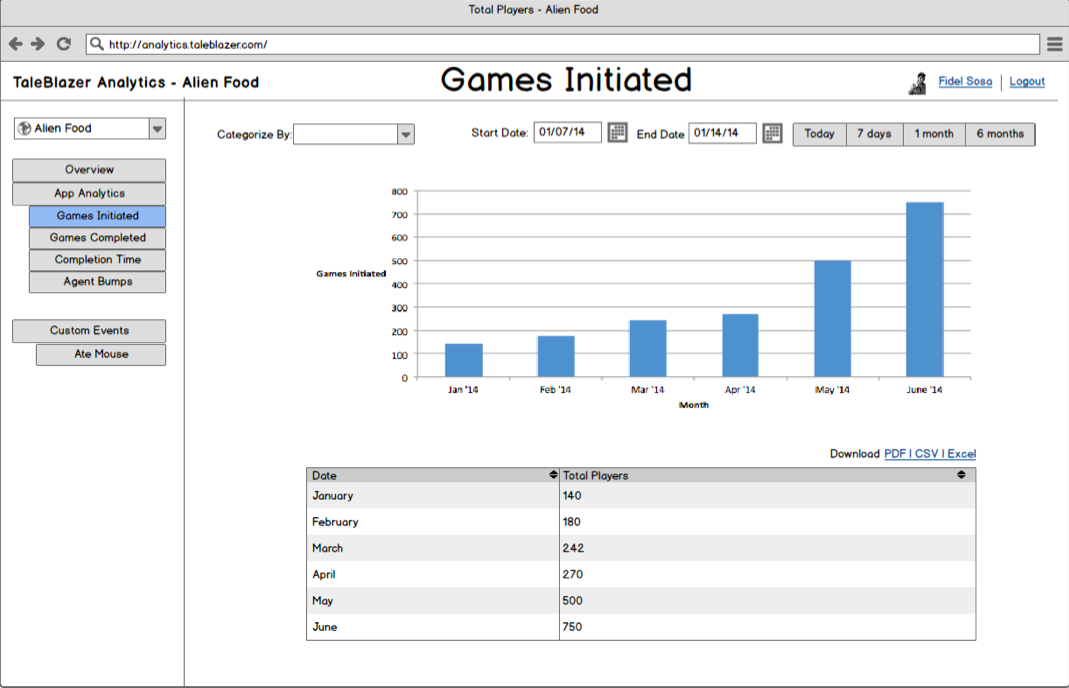
\includegraphics[width=\textwidth]
				{figures/mockup_initiated.png}
			}
	\caption[Early Analytics Site Mockup]{\label{fig:mockup_initiated} Early design for the Games Initiated page, which showed the number of games that were started. This would eventually become the Games Played page in the final site.}
\end{figure}

\subsection{Effect of Mockups on Project Requirements}

In designing the mockups, we were able to determine the set of pages that comprise the TaleBlazer Analytics site. As a direct result, this informed the technical specifications of the project as to the specific types of statistics that would need to be generated from the collected data. For example, early mockups introduced the idea of categorizing information. This feature would go on to become the categorization function, which is an integral part of all statistic calculations in the final TaleBlazer Analytics system. 

From investigating other existing analytics dashboards, features such as fast date range filters were introduced, which live in the final system. The mockups that were created also included features for the future of TaleBlazer Analytics, such as detailed data visualizations. 

\subsection{Partner Feedback}

One of the main goals of creating these mockups was to familiarize our partner institutions with the analytics interface and the functions that would be available to them. In turn, this gave our partners the opportunity to give us feedback regarding desired features, improvements, and changes.

To this end, annotated mockups were sent to our partner institutions along with a short survey. The survey asked our partners to rank the site pages that they foresaw themselves using the most, as well as the categorization options they would most use. This information helped us prioritize development on the most requested pages. Features such as the ability to download the full set of analytics data were a direct result of partner feedback. This feedback also helped us determine how analytics users would use the site. One respondent answered that during game development, they would focus on how often agents were bumped and if the game was completed to help them pinpoint trouble spots. Once the game was stable, they would focus more on how often and when people were playing the game.





